
\subsection{Thick Tangles and Transport Graphs}

Having established a codomain double category, we look towards extending our
notion of TQFTs based on transport graphs in a single manifold to transport
graphs in cobordisms equipped with connections. For simplicity, we only consider
thick tangles equipped with connections, at the moment. Recall that a thick
tangle $X \to Y$ is a smooth surfaces $M$ with boundary $W_0 \amalg W_1$ with
equipped with smooth maps $a_M : X \to M, b_M : Y \to M$ such that $a_M$ and
$b_M$ are diffeomorphisms onto $W_0$ and $W_1$ respectively, and an embedding
$d_M : M \to \R \times [0, 1]$ (satisfying some additional properties, which we
will not need at the moment).

We consider the generating thick tangles equipped with transport graphs.
The following examples of transport graphs in the pair-of-pants, cap and their
duals gives us an idea of the structures we are dealing with:
\[
% Pants:
\begin{tikzpicture}[scale=0.55]
\pants{0, 0}
\lblvert{0, -4}{pants}{\footnotesize pair-of-pants}
\colvert{blue}{-2, 6}{a1}
\lblvert{-2.85, 6}{a1l}{\footnotesize $a_1$}
\colvert{blue}{-2, 4}{a2}
\lblvert{-2.85, 4}{a2l}{\footnotesize $a_2$}
\colvert{blue}{2, 5}{a3}
\lblvert{2.85, 5}{a3l}{\footnotesize $a_3$}
\midarrow{a1}{a3}
\midarrow{a2}{a3}
% Path 1 --> 3
\colvert{blue}{-1.55, 1.65}{a1p}
\lblvert{-1.55, 2.1}{a1pl}{\footnotesize $a_1$}
\colvert{blue}{1.5, -0.75}{a3p1}
\lblvert{1.5, -0.3}{a3p1l}{\footnotesize $a_3$}
\midarrowc{a1p}{0, 1}{0, -1}{a3p1};
% Path 2 --> 3
\colvert{blue}{-1.25, -1.95}{a2p}
\lblvert{-1.25, -1.45}{a2pl}{\footnotesize $a_2$}
\colvert{blue}{1.25, 0.35}{a3p2}
\lblvert{1.25, 0.75}{a3p2l}{\footnotesize $a_3$}
\midarrowc[0.35]{a2p}{0, -2}{1, 0.25}{a3p2}
\end{tikzpicture}
\qquad
% Cap:
\begin{tikzpicture}[scale=0.55]
\capcob{0, 0}
\lblvert{-1.5, -4}{caplbl}{\footnotesize cap}
\colvert{blue}{-2, 5}{a1}
\colvert{green!55!black}{-1, 5}{a2}
\midarrow{a1}{a2}
% Path 1 --> 2
\colvert{blue}{-1.75, 0.75}{a1p}
\colvert{green!55!black}{-1.35, -0.45}{a2p}
\midarrowc{a1p}{-1.75, -0.05}{-1, 0}{a2p}
\end{tikzpicture}
\qquad
% Cup:
\begin{tikzpicture}[scale=0.55]
\cupcob{0, 0}
\lblvert{1.5, -4}{caplbl}{\footnotesize cup}
\colvert{green!55!black}{1, 5}{a1}
\colvert{blue}{2, 5}{a2}
\midarrow{a1}{a2}
% Path 1 --> 2
\colvert{green!55!black}{1.75, 0.75}{a1p}
\colvert{blue}{1.75, -0.75}{a2p}
\midarrowc{a1p}{1.1, 0}{1.1, 0}{a2p}
\end{tikzpicture}
\qquad
% Copants
\begin{tikzpicture}[scale=0.55]
\copants{0, 0}
\lblvert{0, -4}{copants}{\footnotesize co-pair-of-pants}
\colvert{blue}{2, 6}{a1}
\lblvert{2.85, 6}{a1l}{\footnotesize $a_1$}
\colvert{blue}{2, 4}{a2}
\lblvert{2.85, 4}{a2l}{\footnotesize $a_2$}
\colvert{blue}{-2, 5}{a3}
\lblvert{-2.85, 5}{a3l}{\footnotesize $a_3$}
\midarrow{a3}{a1}
\midarrow{a3}{a2}
% Path 3 --> 1
\colvert{blue}{-1.25, 0}{a3p}
\lblvert{-1.25, 0.45}{a3pl}{\footnotesize $a_3$}
\colvert{blue}{1.5, 1.75}{a1p}
\lblvert{1.5, 2.25}{a1pl}{\footnotesize $a_1$}
\midarrowc{a3p}{0, 0}{-0.5, 1}{a1p}
% Path 3 --> 2
\colvert{blue}{1.5, -1.75}{a2p}
\lblvert{1.5, -2.25}{a2pl}{\footnotesize $a_2$}
\midarrowc{a3p}{0, 0}{-0.5, -1}{a2p}
\end{tikzpicture}
\]
We recall that edges that share an end-point need not map to paths that share an
end-point, as we see in the left diagram. At the same time, paths are allowed to
intersect. We also note that we have chosen the pretransport graphs so as to
match their sources and targets with the sources and targets of their realizing
cobordisms. We now turn our attention to the cylinder. We observe that the
cylinder is a cobordism $I \to I$. On the transport graph side, morphisms from a
single blue vertex to another can be any path with blue end-points including the
path consisting of a single blue vertex. However, the gluing unit for the single
blue vertex, on either side, is the single blue vertex itself. Hence, we will
consider the following transport graphs in the cylinder:
\[
\begin{tikzpicture}[scale=0.55]
\idcob{0, 0}
\colvert{blue}{0, 2}{a}
\lblvert{0, -2}{lbl}{\footnotesize cylinder without paths}
\end{tikzpicture}
\qquad \qquad
\begin{tikzpicture}[scale=0.55]
\idcob{0, 0}
\lblvert{0, -2}{lbl}{\footnotesize cylinder with paths}
\colvert{blue}{-2, 2}{a1}
\colvert{blue}{2, 2}{a2}
\midarrow{a1}{a2}
\colvert{blue}{-1.5, -0.15}{a1p}
\colvert{blue}{1.5, 0.15}{a2p}
\midarrowc{a1p}{0, 0.45}{0, -0.45}{a2p}
\end{tikzpicture}
\]

\begin{exm}
We take the example from our first description of the double categorical
approach and adapt it to this setting. The following is one possible diagram:
\[\begin{tikzpicture}[scale=0.33]

\idcobup{1, 0}
\colvert{blue}{-0.5, -1.85}{s}
\colvert{blue}{2, 0.25}{t}
\midarrowc{s}{0, -2}{2, -1}{t}

\coordinate (cntr) at (1, 4);
\pants{cntr}
\colvert{blue}{$(cntr) + (-1.5, 2)$}{s1}
\colvert{blue}{$(cntr) + (-1.5, -2)$}{s2}
\colvert{blue}{$(cntr) + (1.25, 0)$}{t}
\midarrowc{s1}{$(cntr) + (0, 2)$}{$(cntr) + (0, 0)$}{t}
\midarrowc{s2}{$(cntr) + (0, 1)$}{$(cntr) + (0, -1)$}{t}

\coordinate (cntr) at (5, 2);
\pants{cntr}
\colvert{blue}{$(cntr) + (-1.5, 2)$}{s1}
\colvert{blue}{$(cntr) + (-1.5, -2)$}{s2}
\colvert{blue}{$(cntr) + (1.25, 0)$}{t}
\midarrowc{s1}{$(cntr) + (0, 2)$}{$(cntr) + (0, 0)$}{t}
\midarrowc{s2}{$(cntr) + (0, 1)$}{$(cntr) + (0, -1)$}{t}

\coordinate (cntr) at (9, 2);
\begin{scope}[rotate around={180:(cntr)}]
\pants{cntr}
\colvert{blue}{$(cntr) + (-1.5, 2)$}{s1}
\colvert{blue}{$(cntr) + (-1.5, -2)$}{s2}
\colvert{blue}{$(cntr) + (1.25, 0)$}{t}
\midarrowc{s1}{$(cntr) + (0, 2)$}{$(cntr) + (0, 0)$}{t}
\midarrowc{s2}{$(cntr) + (0, 1)$}{$(cntr) + (0, -1)$}{t}
\end{scope}

\coordinate (cntr) at (13, 2);
\pants{cntr}
\colvert{blue}{$(cntr) + (-1.5, 2)$}{s1}
\colvert{blue}{$(cntr) + (-1.5, -2)$}{s2}
\colvert{blue}{$(cntr) + (1.25, 0)$}{t}
\midarrowc{s1}{$(cntr) + (0, 2)$}{$(cntr) + (0, 0)$}{t}
\midarrowc{s2}{$(cntr) + (0, 1)$}{$(cntr) + (0, -1)$}{t}

\coordinate (cntr) at (17, 2);
\begin{scope}[rotate around={180:(cntr)}]
\pants{cntr}
\colvert{blue}{$(cntr) + (-1.5, 2)$}{s1}
\colvert{blue}{$(cntr) + (-1.5, -2)$}{s2}
\colvert{blue}{$(cntr) + (1.25, 0)$}{t}
\midarrowc{s1}{$(cntr) + (0, 2)$}{$(cntr) + (0, 0)$}{t}
\midarrowc{s2}{$(cntr) + (0, 1)$}{$(cntr) + (0, -1)$}{t}
\end{scope}

\coordinate (cntr) at (21, 2);
\pants{cntr}
\colvert{blue}{$(cntr) + (-1.5, 2)$}{s1}
\colvert{blue}{$(cntr) + (-1.5, -2)$}{s2}
\colvert{blue}{$(cntr) + (1.25, 0)$}{t}
\midarrowc{s1}{$(cntr) + (0, 2)$}{$(cntr) + (0, 0)$}{t}
\midarrowc{s2}{$(cntr) + (0, 1)$}{$(cntr) + (0, -1)$}{t}

\coordinate (cntr) at (25, 2);
\begin{scope}[rotate around={180:(cntr)}]
\pants{cntr}
\colvert{blue}{$(cntr) + (-1.5, 2)$}{s1}
\colvert{blue}{$(cntr) + (-1.5, -2)$}{s2}
\colvert{blue}{$(cntr) + (1.25, 0)$}{t}
\midarrowc{s1}{$(cntr) + (0, 2)$}{$(cntr) + (0, 0)$}{t}
\midarrowc{s2}{$(cntr) + (0, 1)$}{$(cntr) + (0, -1)$}{t}
\end{scope}

\end{tikzpicture}\]
\end{exm}

\begin{exm}
We need not consider transport graphs that match the pair-of-pants or the
cylinder (or their duals) exactly. For instance, we could consider the following
graph:
\[\begin{tikzpicture}[scale=0.5]
\coordinate (cntr) at (1, 4);
\pants{cntr}
\colvert{blue}{$(cntr) + (-1.5, 2)$}{s1}
\colvert{blue}{$(cntr) + (-1.5, -2)$}{s2}
\colvert{green!55!black}{$(cntr) + (0, 1)$}{t1}
\colvert{blue}{$(cntr) + (0, -1)$}{t2}
\colvert{blue}{$(cntr) + (1.5, -0.5)$}{t3}
\midarrowc{s1}{$(cntr) + (0, 2)$}{$(cntr) + (-1, 1)$}{t1}
\midarrowc[0.33]{s2}{$(cntr) + (-0.25, -1)$}{$(cntr) + (0, 1)$}{t1}
\midarrowc{s1}{$(cntr) + (-0.5, 0)$}{$(cntr) + (-0.5, 2)$}{t2}
\midarrowc{s2}{$(cntr) + (-0.5, -2)$}{$(cntr) + (-0.5, -1)$}{t2}
\midarrowc{t1}{$(cntr) + (0.5, 0)$}{$(cntr) + (1, 0.5)$}{t3}
\midarrowc{t2}{$(cntr) + (0.5, 0.5)$}{$(cntr) + (1, -0.5)$}{t3}
\end{tikzpicture}\]
Notice that the source and target of the graph matches the source and target of
the pair-of-pants event though the graph is not a pair-of-pants graph. Also
notice that this graph has an internal green vertex.
\end{exm}

From these examples, we are motiviated to note the following definition.
\begin{defn}
Given a $2$--dimensional thick tangle, consider a transport graph in
the tangle such that the source of the graph has the same number of vertices
as the number of boundary components of the source of the tangle and the
colouring and ordering of the source of the graph is such that a blue vertex
corresponds to an interval boundary component and a green vertex corresponds to
an empty boundary component. Furthermore, that the analogous statement holds for
the targets of the graph and the tangle. We then call the given transport graph
admissible for the given tangle.
\end{defn}

An immediate corollary of this definition is:
\begin{cor}
Admissible transport graphs in gluable thick tangles are gluable.
\end{cor}

The examples we have seen so far are all admissible. We also show graphs that
are not admissible in the following example.

\begin{exm}
The following are not admissible transport graphs:
\[\begin{tikzpicture}[scale=0.33]

\coordinate (cntr) at (1, 4);
\pants{cntr}
\colvert{blue}{$(cntr) + (-1.5, 2)$}{s}
\colvert{blue}{$(cntr) + (1.5, 0)$}{t}
\midarrow{s}{t}
\lblvert{$(cntr) + (0, -5)$}{lbl}{\small not enough}
\lblvert{$(cntr) + (0, -6)$}{lbl}{\small source vertices}

\coordinate (cntr) at (11, 4);
\idcob{cntr}
\colvert{green!55!black}{$(cntr) + (-1.5, 0)$}{s}
\colvert{blue}{$(cntr) + (1.5, 0)$}{t}
\midarrow{s}{t}
\lblvert{$(cntr) + (0, -5)$}{lbl}{\small source should}
\lblvert{$(cntr) + (0, -6)$}{lbl}{\small be blue}

\coordinate (cntr) at (21, 4);
\copants{cntr}
\capcob{$(cntr) + (4, 2)$}
\colvert{blue}{$(cntr) + (-1.5, 0)$}{s}
\colvert{blue}{$(cntr) + (2.5, 2)$}{t1}
\colvert{blue}{$(cntr) + (1.5, -2)$}{t2}
\midarrow{s}{t1}
\midarrow{s}{t2}
\lblvert{$(cntr) + (0, -5)$}{lbl}{\small top traget}
\lblvert{$(cntr) + (0, -6)$}{lbl}{\small should be}
\lblvert{$(cntr) + (0, -7.25)$}{lbl}{\small green}

\end{tikzpicture}\]
\end{exm}

So far, we have only shown the diagrams of surfaces with paths in these examples
but what we need to work with are surfaces equipped with bundles, connections
and transport graphs. We will now construct a monoidal double category
consisting of these structures.

Consider the monoidal double category $\CConn^V_{\DThick}$ of gluable
connections on gluable $V$--fibred (smooth or complex) bundles on
$2$--dimensional thick tangles.
For each horizontal $1$--morphism (bundle with connection) in this category, we
take all admissible transport graphs in the base of the bundle such that all
paths consist only of points internal to the base space and away from the
boundary collar over which the bundle has been made trivial.

For each gluable bundle equipped with a gluable connection and an admissible
transport graph in this manner, we take its source to be the source of the
bundle in $\CConn^V_{\DThick}$ along with the source of the transport graph.
Targets are defined similarly. The gluing units are the disjoint unions of
cylinders of the following form shown before:
\[\begin{tikzpicture}[scale=0.55]
\idcob{0, 0}
\colvert{blue}{0, 2}{a}
\lblvert{0, -2}{lbl}{\footnotesize cylinder without paths}
\end{tikzpicture}\]

Naturally, the object category consists of the sources and targets of the
horizontal $1$--morphisms and transport isomorphisms between them that are also
connection isomorphisms -- similar to the monoidal double category $\TG(M)$ of
transport graphs in a manifold $M$ defined in subsection
\ref{subsec:one_man_tqft}. The morphism category consists of the horizontal
$1$--morphisms along with transport isomorphisms that are also connection
isomorphisms. Finally, monoidal structure is given by disjoint union, as
expected.

Having the developed the basic idea of such a monoidal double category, we avoid
going into further detail because it does not provide any additional insight. We
simply note that the structure outlined here is a monoidal double category that
can serve as the domain for a notion of (double) functorial quantum field
theory. Hence, we end this subsection with the following definition.

\begin{defn}
The monoidal double category outlined above is called the double category of
transport graphs in $2$--dimensional thick tangles over $V$ and is
denoted $\TG\br{\CConn^V_{\DThick}}$.
\end{defn}

